\section{Módulo de Registro}

	O Módulo de Registro é responsável por cadastrar novos usuários no sistema e treiná-lo para também reconhecer esse novo usuário. Basicamente, o processo de registro, ilustrado na Figura~\ref{fig:registro}, segue as seguintes etapas :

		\begin{figure}[htb]
			\begin{center}
				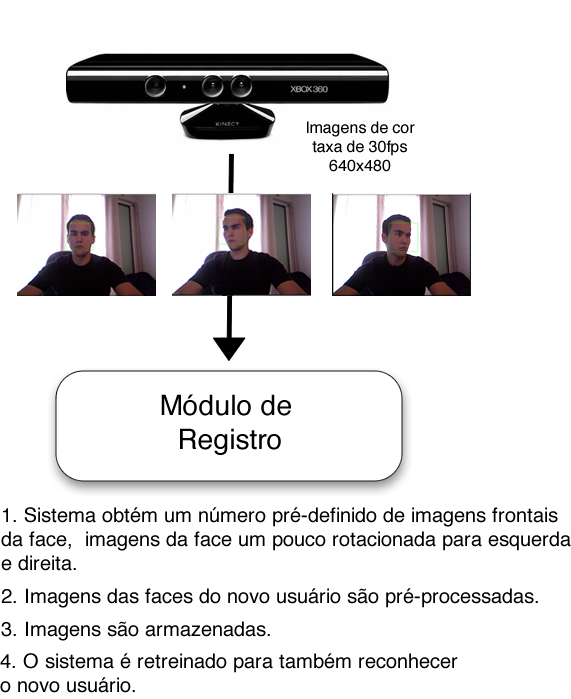
\includegraphics[scale=1.5]{figuras/4.ProblemaEProposta/registro.png}
			\end{center}
			\caption{Módulo de Registro do Sistema TRUE.}
			\label{fig:registro}
		\end{figure}		

		\begin{enumerate}
			\item Obtenção das imagens do novo usuário.
			\item Processamento das imagens, isto é, as imagens são convertidas em escala de cinza, novas imagens são criadas recortando a região da face encontrada. Em seguida, as imagens são redimensionadas e equalizadas criando assim padrões de tamanho, brilho e contraste.
			\item Armazenamento das imagens.
			\item Treinamento do sistema para reconhecer esse usuário.
		\end{enumerate}

	A última etapa do módulo de registro consiste no treinamento do sistema. O treinamento inicia-se liberando os atuais dados de treinamento. Então, um vetor de imagens é obtido lendo todas as imagens contidas no banco de faces. Através deste vetor, obtém-se a \textit{eigenface} média, os \textit{eigenfaces} e os \textit{eigenvalues}. Estes últimos são normalizados. Para cada usuário cadastrado no Sistema TRUE, suas imagens são projetadas no subespaço através do método PCA (\textit{Principal Component Analisys} - Análise de Componente Principal), que reduz suas dimensionalidades, e são calculdas suas distâncias em relação aos \textit{eigenfaces} obtendo um vetor de distâncias. Os \textit{eigenfaces}, os \textit{eigenvalues}, a \textit{eigenface} média e os vetores de distâncias são armazenados e podem ser utilizados pelo Módulo de Reconhecimento. A Figura~\ref{fig:treinamento} mostra essas etapas de treinamento.

		\begin{figure}[htb]
			\begin{center}
				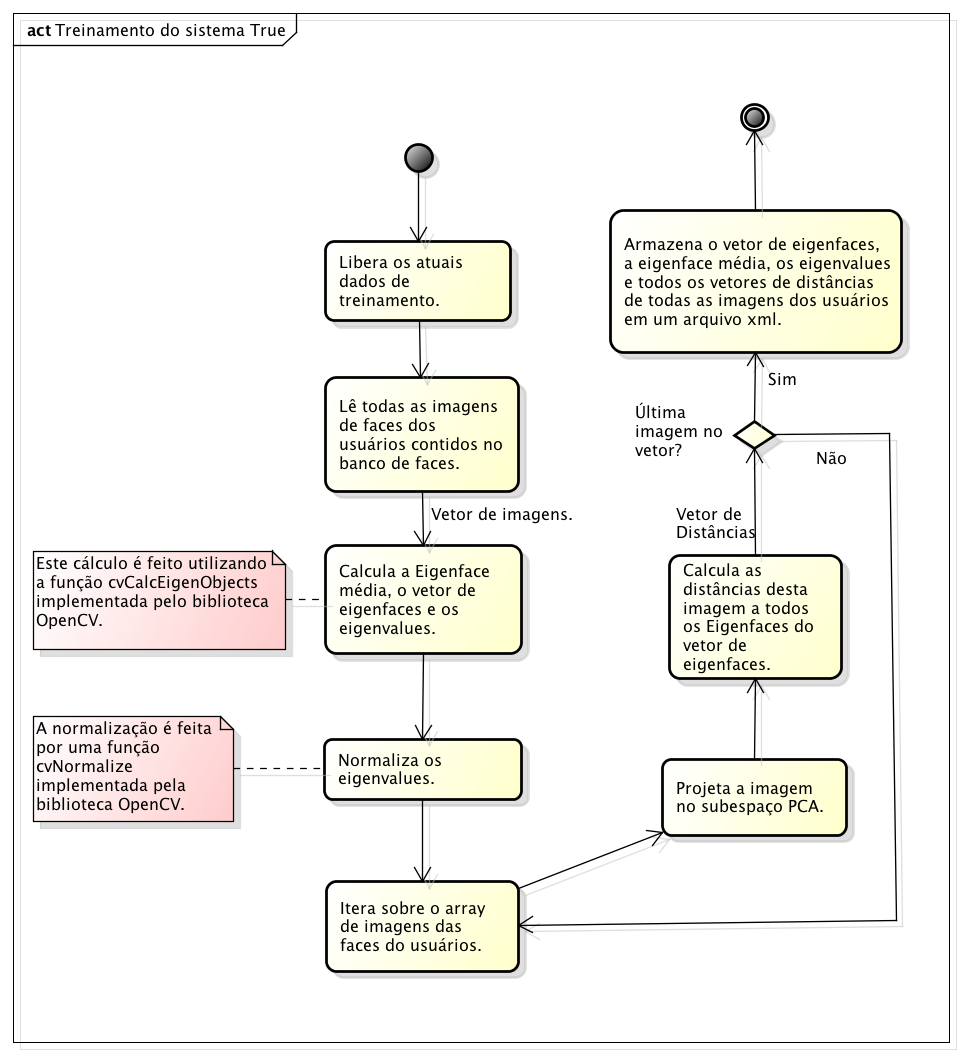
\includegraphics[scale=0.5]{figuras/4.ProblemaEProposta/diagrama-registro.png}
			\end{center}
			\caption{Fluxo básico do treinamento do Sistema TRUE.}
			\label{fig:treinamento}
		\end{figure}	

	Após o treinamento, o Sistema TRUE é reiniciado para que o reconhecimento seja feito utilizando as novas imagens e informações obtidas com o treinamento.